\section{Experimental Method}

No experiments were carried out for this report, but measurements from previous students are used. The experimental set-up that they used and the computer algorithms that were used for this report will be discussed in this section.

\subsection{Experimental set-up}

\begin{wrapfigure}{r}{0.6\textwidth}
    \centering
    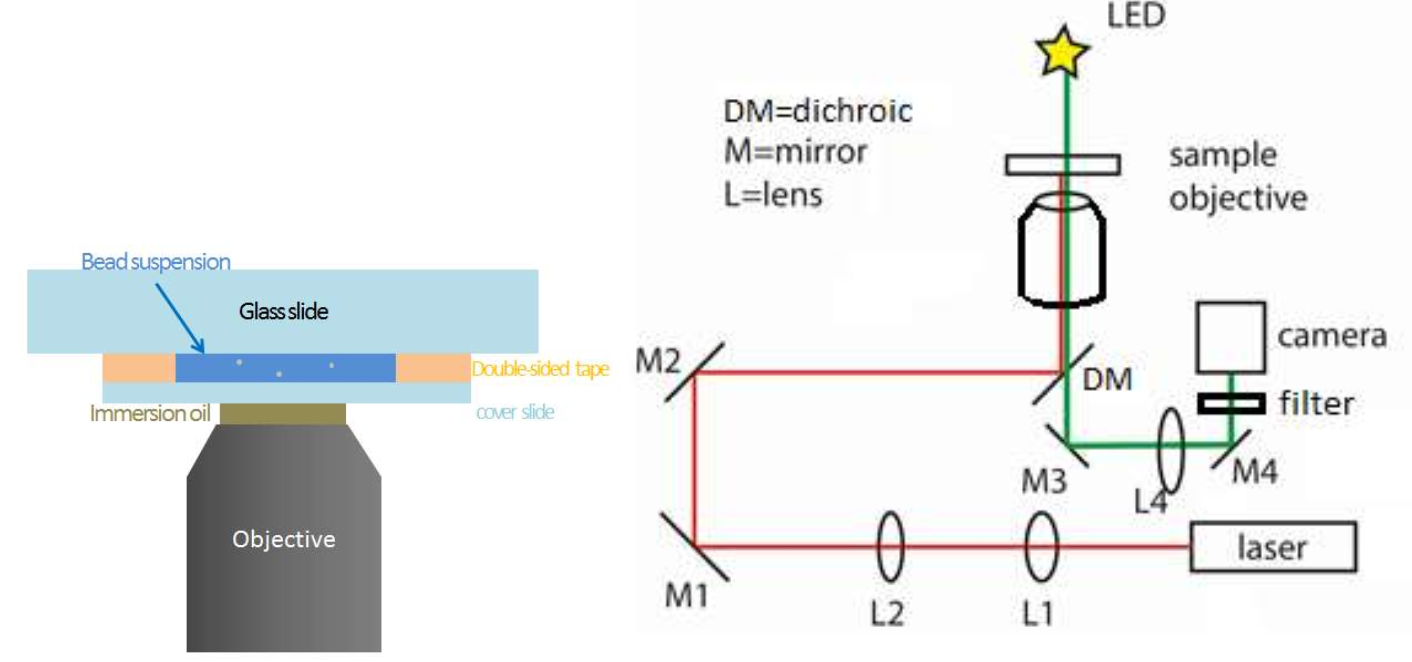
\includegraphics[width=0.55\textwidth,keepaspectratio]{figures/setup.png}
    \caption{Schematic diagram of the experimental set-up that was used for the experiments corresponding with the treated data in this report. This diagram was taken from the practicum manual \cite{practicum_manual}.}
    \label{fig_setup}
\end{wrapfigure}


The experimental set-up that was used for this report can be seen in figure \ref{fig_setup}.
According to the practicum manual, the red light from the laser has a wavelength of$\lambda=658$ nm and passes through a beam expander in order to completely fill the back (back focal plane) of the objective.
The beads that are used in the experiment have a diameter of approximately $ 2 \mu m$.
The mirrors M1 and M2 are used for compacting the beam path and aligning the beam to the optical axis of the objective.
The used objective is meant to be used in an infinity corrected microscope.
L4 focusses the light back to an image at focal distance.
In the set-up, the L1 and L2 have focal length of respectively 50 and 350 mm. The front focal distance of the objective lens is 1.8 mm and the second objective lens has a focal length of 200 mm. Using simple division and equation \ref{eq_error} we find that the magnification is  $ M = \frac{200}{1.8} = 1.1  \: \pm 0.3 \cdot 10^2$. Given the pixel size of the camera of $ 5.2 \: \mu $  and equation  \ref{eq_error} we find that the conversion factor for pixels to length is given by $l_{pixel} = \frac{5.2}{M} \cdot 10^{-6} \approx 4.7 \; \pm 0.1 \; \cdot 10^{-8} m/pixel$.

Using the discussed set-up, a bead was to be trapped by a laser beam and images were taken at fixed time intervals. This was performed for laser beams with different powers. The involved powers were 0, 5, 10, 20, 30 and 40 mW. For this report, two data sets from different students are analysed.

\subsection{Computation}

A MATLAB algorithm was provided for this practical in order to calculate the trap constant in a x- and y-direction, $k_{trap,x}$ and $k_{trap,y}$. This algorithm involves noise removal of the images and tracking the bead using a 'quadrant-interpolation (QI) algorithm  which makes use of the circular geometry of the diffraction pattern to resample the image on a circular grid.' \cite{loenhout} Subsequently, power spectrum analysis is performed to calculate the values for $k_{trap,x}$ and $k_{trap,y}$. Using this MATLAB code and a linear regression method, the correlation between the laser power and the trap constants are determined for the two data sets.

Secondly, a PYTHON algorithm is used with the same noise cancelling technique, but with a trackpy function to follow the bead. This algorithm subsequently calculates the covariance matrix and the vectors describing the covariance ellipse. Using this PYTHON code, the change of this covariance ellipse is analysed.



